% Options for packages loaded elsewhere
% Options for packages loaded elsewhere
\PassOptionsToPackage{unicode}{hyperref}
\PassOptionsToPackage{hyphens}{url}
\PassOptionsToPackage{dvipsnames,svgnames,x11names}{xcolor}
%
\documentclass[
  letterpaper,
  DIV=11,
  numbers=noendperiod]{scrartcl}
\usepackage{xcolor}
\usepackage{amsmath,amssymb}
\setcounter{secnumdepth}{-\maxdimen} % remove section numbering
\usepackage{iftex}
\ifPDFTeX
  \usepackage[T1]{fontenc}
  \usepackage[utf8]{inputenc}
  \usepackage{textcomp} % provide euro and other symbols
\else % if luatex or xetex
  \usepackage{unicode-math} % this also loads fontspec
  \defaultfontfeatures{Scale=MatchLowercase}
  \defaultfontfeatures[\rmfamily]{Ligatures=TeX,Scale=1}
\fi
\usepackage{lmodern}
\ifPDFTeX\else
  % xetex/luatex font selection
\fi
% Use upquote if available, for straight quotes in verbatim environments
\IfFileExists{upquote.sty}{\usepackage{upquote}}{}
\IfFileExists{microtype.sty}{% use microtype if available
  \usepackage[]{microtype}
  \UseMicrotypeSet[protrusion]{basicmath} % disable protrusion for tt fonts
}{}
\makeatletter
\@ifundefined{KOMAClassName}{% if non-KOMA class
  \IfFileExists{parskip.sty}{%
    \usepackage{parskip}
  }{% else
    \setlength{\parindent}{0pt}
    \setlength{\parskip}{6pt plus 2pt minus 1pt}}
}{% if KOMA class
  \KOMAoptions{parskip=half}}
\makeatother
% Make \paragraph and \subparagraph free-standing
\makeatletter
\ifx\paragraph\undefined\else
  \let\oldparagraph\paragraph
  \renewcommand{\paragraph}{
    \@ifstar
      \xxxParagraphStar
      \xxxParagraphNoStar
  }
  \newcommand{\xxxParagraphStar}[1]{\oldparagraph*{#1}\mbox{}}
  \newcommand{\xxxParagraphNoStar}[1]{\oldparagraph{#1}\mbox{}}
\fi
\ifx\subparagraph\undefined\else
  \let\oldsubparagraph\subparagraph
  \renewcommand{\subparagraph}{
    \@ifstar
      \xxxSubParagraphStar
      \xxxSubParagraphNoStar
  }
  \newcommand{\xxxSubParagraphStar}[1]{\oldsubparagraph*{#1}\mbox{}}
  \newcommand{\xxxSubParagraphNoStar}[1]{\oldsubparagraph{#1}\mbox{}}
\fi
\makeatother


\usepackage{longtable,booktabs,array}
\usepackage{calc} % for calculating minipage widths
% Correct order of tables after \paragraph or \subparagraph
\usepackage{etoolbox}
\makeatletter
\patchcmd\longtable{\par}{\if@noskipsec\mbox{}\fi\par}{}{}
\makeatother
% Allow footnotes in longtable head/foot
\IfFileExists{footnotehyper.sty}{\usepackage{footnotehyper}}{\usepackage{footnote}}
\makesavenoteenv{longtable}
\usepackage{graphicx}
\makeatletter
\newsavebox\pandoc@box
\newcommand*\pandocbounded[1]{% scales image to fit in text height/width
  \sbox\pandoc@box{#1}%
  \Gscale@div\@tempa{\textheight}{\dimexpr\ht\pandoc@box+\dp\pandoc@box\relax}%
  \Gscale@div\@tempb{\linewidth}{\wd\pandoc@box}%
  \ifdim\@tempb\p@<\@tempa\p@\let\@tempa\@tempb\fi% select the smaller of both
  \ifdim\@tempa\p@<\p@\scalebox{\@tempa}{\usebox\pandoc@box}%
  \else\usebox{\pandoc@box}%
  \fi%
}
% Set default figure placement to htbp
\def\fps@figure{htbp}
\makeatother





\setlength{\emergencystretch}{3em} % prevent overfull lines

\providecommand{\tightlist}{%
  \setlength{\itemsep}{0pt}\setlength{\parskip}{0pt}}



 


\usepackage{booktabs}
\usepackage{longtable}
\usepackage{array}
\usepackage{multirow}
\usepackage{wrapfig}
\usepackage{float}
\usepackage{colortbl}
\usepackage{pdflscape}
\usepackage{tabu}
\usepackage{threeparttable}
\usepackage{threeparttablex}
\usepackage[normalem]{ulem}
\usepackage{makecell}
\usepackage{xcolor}
\KOMAoption{captions}{tableheading}
\makeatletter
\@ifpackageloaded{caption}{}{\usepackage{caption}}
\AtBeginDocument{%
\ifdefined\contentsname
  \renewcommand*\contentsname{Table of contents}
\else
  \newcommand\contentsname{Table of contents}
\fi
\ifdefined\listfigurename
  \renewcommand*\listfigurename{List of Figures}
\else
  \newcommand\listfigurename{List of Figures}
\fi
\ifdefined\listtablename
  \renewcommand*\listtablename{List of Tables}
\else
  \newcommand\listtablename{List of Tables}
\fi
\ifdefined\figurename
  \renewcommand*\figurename{Figure}
\else
  \newcommand\figurename{Figure}
\fi
\ifdefined\tablename
  \renewcommand*\tablename{Table}
\else
  \newcommand\tablename{Table}
\fi
}
\@ifpackageloaded{float}{}{\usepackage{float}}
\floatstyle{ruled}
\@ifundefined{c@chapter}{\newfloat{codelisting}{h}{lop}}{\newfloat{codelisting}{h}{lop}[chapter]}
\floatname{codelisting}{Listing}
\newcommand*\listoflistings{\listof{codelisting}{List of Listings}}
\makeatother
\makeatletter
\makeatother
\makeatletter
\@ifpackageloaded{caption}{}{\usepackage{caption}}
\@ifpackageloaded{subcaption}{}{\usepackage{subcaption}}
\makeatother
\usepackage{bookmark}
\IfFileExists{xurl.sty}{\usepackage{xurl}}{} % add URL line breaks if available
\urlstyle{same}
\hypersetup{
  pdftitle={Bern25 summary charts},
  colorlinks=true,
  linkcolor={blue},
  filecolor={Maroon},
  citecolor={Blue},
  urlcolor={Blue},
  pdfcreator={LaTeX via pandoc}}


\title{Bern25 summary charts}
\author{}
\date{}
\begin{document}
\maketitle

\subsection{The scope of the
reporting}\label{the-scope-of-the-reporting}

There were altogether 72 \emph{species} and 6 \emph{habitat types}
involved in the assessment (Table~\ref{tbl-fgrp}). Species and habitat
types are collectively called \emph{features} so there were altogether
78 features assessed. (\emph{TODO: explain BGRs, assessments (feature x
BGR), Emerald, etc\ldots{}})

\begin{table}

\caption{\label{tbl-fgrp}}

\centering{

\centering
\caption{\label{tab:tbl-fgrp}Groups of features (species, habitats) used in this report (Nf: number of features, Na1: number of full assessments, Na2: number of partial assessments)}
\centering
\begin{tabular}[t]{l|c|c|c}
\hline
Feature group & Nf & Na1 & Na2\\
\hline
Mammals (ma) & 7 & 25 & 0\\
\hline
Fishes \& amphibians (fa) & 6 & 15 & 0\\
\hline
Insects and molluscs (im) & 14 & 23 & 3\\
\hline
Vascular plants (vp) & 33 & 47 & 5\\
\hline
Mosses (mo) & 12 & 31 & 1\\
\hline
Habitat types (ht) & 6 & 17 & 0\\
\hline
Total & 78 & 158 & 9\\
\hline
\end{tabular}

}

\end{table}%

\subsection{Conservation status of species and habitat
types}\label{conservation-status-of-species-and-habitat-types}

We start with presenting an overview of the conclusions of the
assessments. Each assessment has an overall conclusion, which is based
on four ``parameters'', each of which has its own conclusions. The
conclusions for the individual parameters rely on quantitative and
qualitative data collected by taxonomic experts following detailed
guidelines provided by the Bern Secretariat. The four assessment
parameters for species include its \emph{distribution range} (Ran),
\emph{population size} (Pop), the quality and quantity of the
\emph{available habitat} for the species (H4s), and its \emph{future
prospects} (Fpr) based on the balance of pressures and conservation
measures. All conclusions are evaluated in a simple ``traffic light
system'' using one of the following four \emph{conservation status}
categories:

\begin{itemize}
\tightlist
\item
  \textbf{FV}: Favourable (green),
\item
  \textbf{U1}: Unfavourable - inadequate (amber),
\item
  \textbf{U2}: Unfavourable - bad (red),
\item
  \textbf{XX}: Unknown (grey).
\end{itemize}

\subsubsection{Species assessments}\label{species-assessments}

Table~\ref{tbl-conclusions-sp-fgrp} provides an overview of the overall
conclusions across the major species groups, whereas
Table~\ref{tbl-conclusions-sp-para} shows the distribution of the
partial conclusions for the individual parameters across all the
species.

\begin{table}

\caption{\label{tbl-conclusions-sp-fgrp}}

\centering{

\centering
\caption{\label{tab:tbl-conclusions-sp-fgrp}Distribution of overall conclusions across the different groups of features (FV: Favourable; U1: Unfavourable - inadequate; U2: Unfavourable - bad; XX: Unknown)}
\centering
\begin{tabular}[t]{l|c|c|c|c}
\hline
Species group & FV & U1 & U2 & XX\\
\hline
Mammals (ma) & 3 & 20 & 2 & -\\
\hline
Fishes \& amphibians (fa) & - & 3 & 3 & 9\\
\hline
Insects and molluscs (im) & 3 & 6 & 8 & 6\\
\hline
Vascular plants (vp) & 1 & 26 & 18 & 2\\
\hline
Mosses (mo) & 5 & 15 & 11 & -\\
\hline
All (all) & 12 & 70 & 42 & 17\\
\hline
\end{tabular}

}

\end{table}%

\begin{table}

\caption{\label{tbl-conclusions-sp-para}}

\centering{

\centering
\caption{\label{tab:tbl-conclusions-sp-para}Distribution of partial conclusions over the different parameters (FV: Favourable; U1: Unfavourable - inadequate; U2: Unfavourable - bad; XX: Unknown)}
\centering
\begin{tabular}[t]{l|c|c|c|c}
\hline
Assessment parameters & FV & U1 & U2 & XX\\
\hline
Range (Ran) & 48 & 54 & 14 & 25\\
\hline
Population (Pop) & 15 & 83 & 11 & 32\\
\hline
Habitat for species (H4s) & 41 & 50 & 33 & 17\\
\hline
Future prospects (Fpr) & 14 & 68 & 39 & 20\\
\hline
\end{tabular}

}

\end{table}%

Below we also visualise the distribution of the conclusions across the
different species groups and assessment parameters
(Figure~\ref{fig-sp-conclusions}).

\begin{figure}

\begin{minipage}{0.50\linewidth}

\pandocbounded{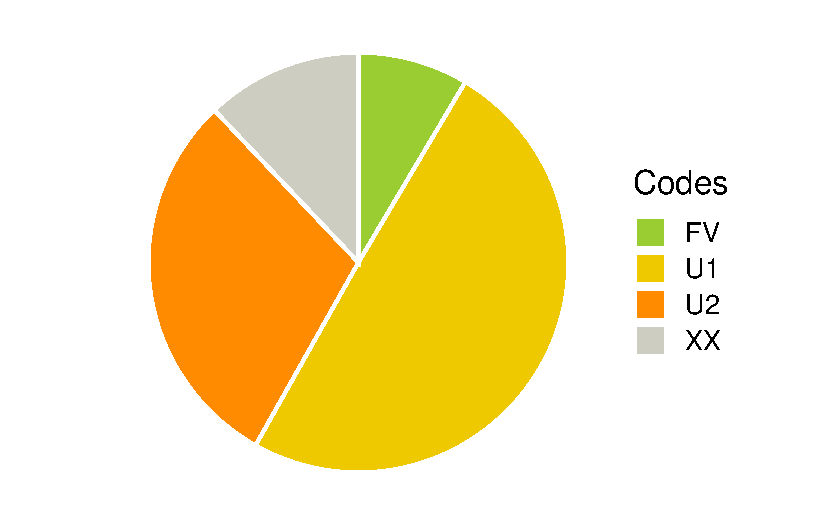
\includegraphics[keepaspectratio]{analyse_data_main_files/figure-pdf/conclusions_1a-1.pdf}}

\end{minipage}%
%
\begin{minipage}{0.50\linewidth}

\pandocbounded{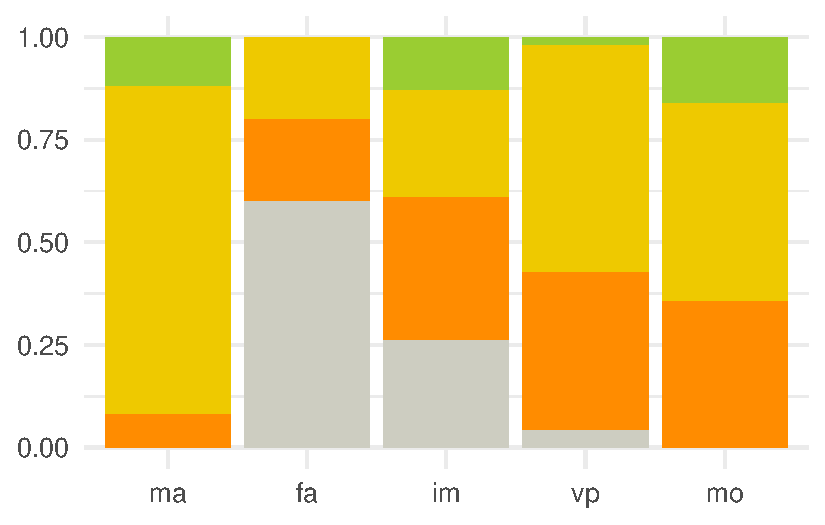
\includegraphics[keepaspectratio]{analyse_data_main_files/figure-pdf/conclusions_1b-1.pdf}}

\end{minipage}%
\newline
\begin{minipage}{0.25\linewidth}

\pandocbounded{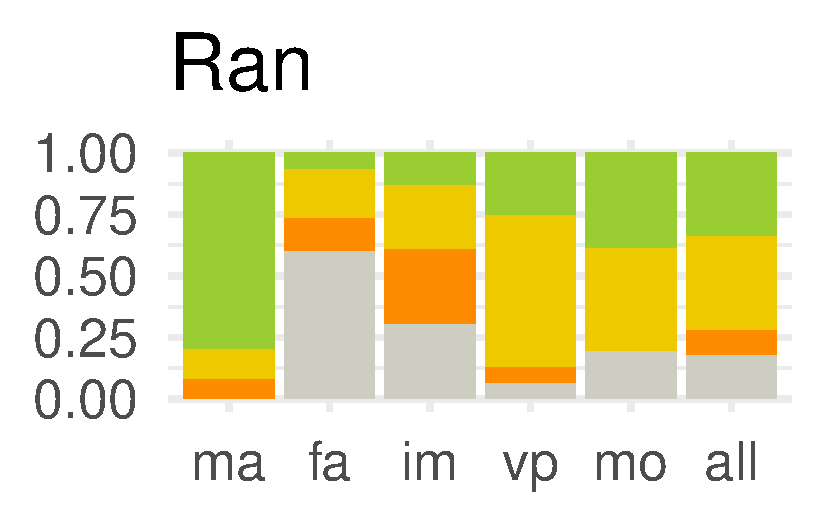
\includegraphics[keepaspectratio]{analyse_data_main_files/figure-pdf/conclusions_2a-1.pdf}}

\end{minipage}%
%
\begin{minipage}{0.25\linewidth}

\pandocbounded{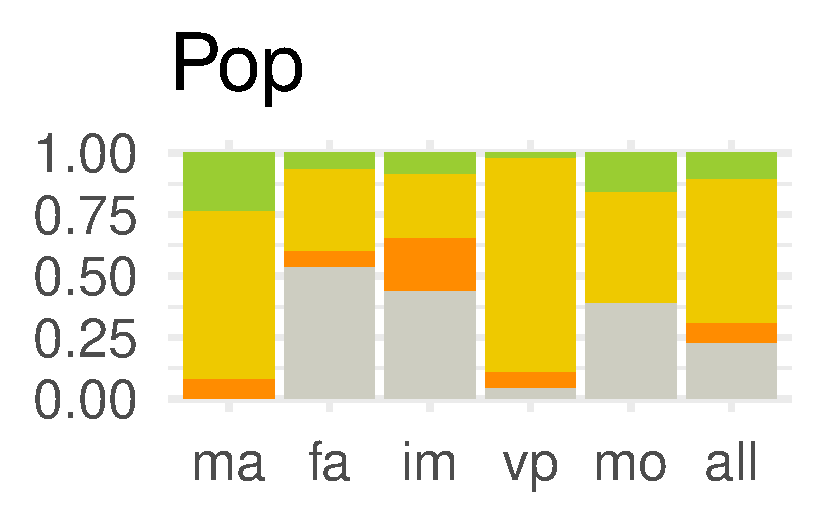
\includegraphics[keepaspectratio]{analyse_data_main_files/figure-pdf/conclusions_2b-1.pdf}}

\end{minipage}%
%
\begin{minipage}{0.25\linewidth}

\pandocbounded{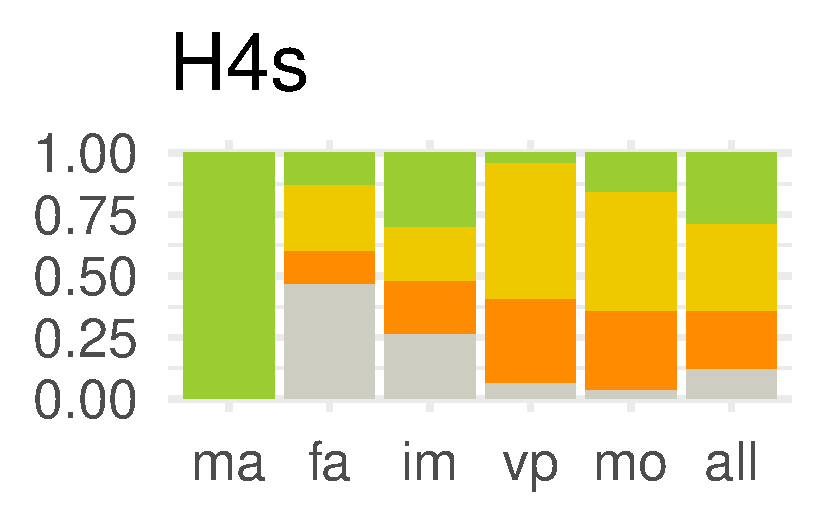
\includegraphics[keepaspectratio]{analyse_data_main_files/figure-pdf/conclusions_2c-1.pdf}}

\end{minipage}%
%
\begin{minipage}{0.25\linewidth}

\pandocbounded{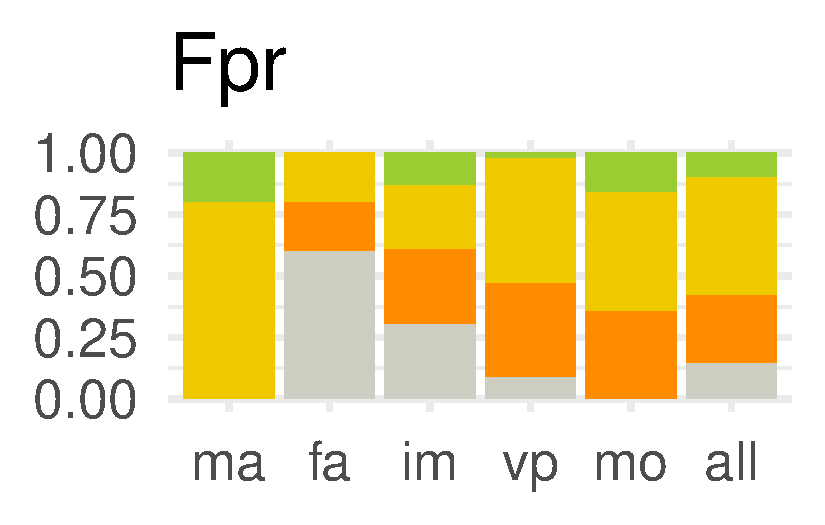
\includegraphics[keepaspectratio]{analyse_data_main_files/figure-pdf/conclusions_2d-1.pdf}}

\end{minipage}%

\caption{\label{fig-sp-conclusions}The conclusions of the species
assessments in the 2025 reporting of Norway to the Bern Convention
(Resultion 8). Top row: overall conclusions for all species (pie chart)
and for major species groups (columns). Bottom row: partial conclusions
for the four main assessment parameters.}

\end{figure}%

\subsubsection{Habitat type assessments}\label{habitat-type-assessments}

Table~\ref{tbl-conclusions-ha-para} and Figure~\ref{fig-ha-conclusions}
provide an overview of the different conclusions for the habitat types
assessed in 2025 in Norway.

\begin{table}

\caption{\label{tbl-conclusions-ha-para}}

\centering{

\centering
\caption{\label{tab:tbl-conclusions-ha-para}Distribution of partial conclusions over the different parameters (FV: Favourable; U1: Unfavourable - inadequate; U2: Unfavourable - bad; XX: Unknown)}
\centering
\begin{tabular}[t]{l|c|c|c}
\hline
Assessment parameters & FV & U2 & U1\\
\hline
Range (Ran) & 15 & 2 & -\\
\hline
Area of habitats (Are) & - & 8 & 9\\
\hline
Structure and function (SnF) & - & 12 & 5\\
\hline
Future prospects (Fpr) & - & 12 & 5\\
\hline
Overall conclusion (OvC) & - & 12 & 5\\
\hline
\end{tabular}

}

\end{table}%

\begin{figure}

\begin{minipage}{0.50\linewidth}

\pandocbounded{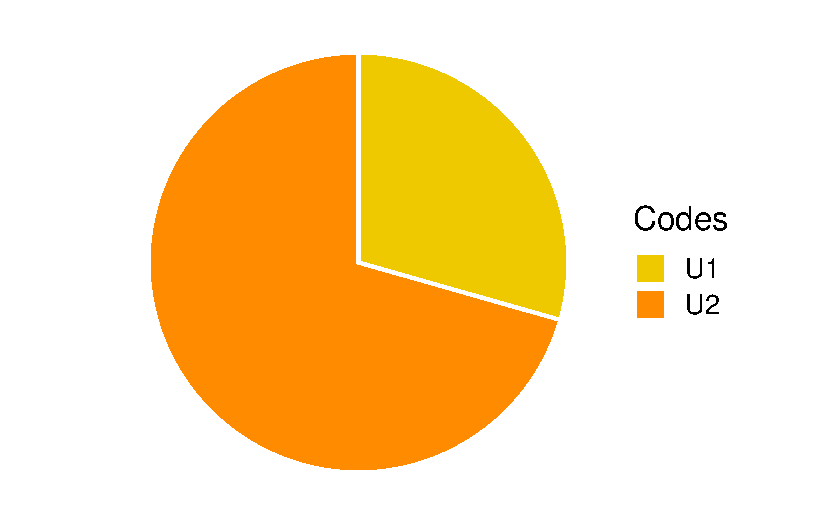
\includegraphics[keepaspectratio]{analyse_data_main_files/figure-pdf/conclusions_ha1-1.pdf}}

\end{minipage}%
%
\begin{minipage}{0.50\linewidth}

\pandocbounded{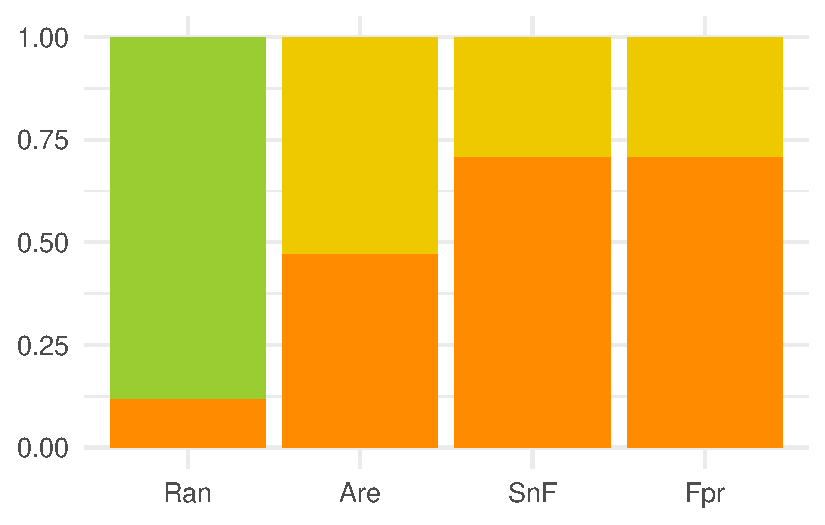
\includegraphics[keepaspectratio]{analyse_data_main_files/figure-pdf/conclusions_ha2-1.pdf}}

\end{minipage}%

\caption{\label{fig-ha-conclusions}The conclusions of habitat type
assessments in the 2025 reporting of Norway to the Bern Convention
(Resultion 8). Left: overall conclusions for all habitat types (pie
chart); right: partial conclusions for the four main assessment
parameters (Ran: range, Are: area, SnF: structure and function, Fpr:
future prospects)}

\end{figure}%

\subsection{Changes and trends}\label{changes-and-trends}

The assessment protocol offers several ways to describe past, present
and future trends in the conservation status of the studied species and
habitats. This includes the assessment of the \emph{short-term} and
\emph{long-term} trends by the experts participating in the 2025
assessment, as well as a direct comparisons of the consecutive
assessments (e.g comparing the conservation status of the same species
\& habitats assessed in 2019 and 2025). In the context of the Bern
Convention \emph{short-term trends} always refer to the past 12 years
(i.e.~2013-2024 in this case), whereas \emph{long term trends} are
referring to the 24 year period before the assessment date
(i.e.~2001-2024). In addition, the parameter \emph{future prospects}
discussed in the previous section also addresses trends, synthesizing
expectations for changes in the other three parameters during the
forthcoming 12 years (i.e.~2025-2036).

In the next few sections we provide an overview of the main current and
past trends relying on the different elements of the Bern assessment
protocol.

\subsubsection{Short term trends}\label{short-term-trends}

Short term trends are first assessed individually for the different
state parameters (range, population size, and habitat availability for
species, and range, area, and structure/function for habitat types), and
then the directions of these elementary trends are aggregated into an
\emph{overall trend qualifier}, which is the second flagship output of
Bern Convention assessments, providing critical insights for the
interpretation of the \emph{overall conservation status}. In
Figure~\ref{fig-trend-qualifiers} we provide an overview of these trend
qualifiers for the different groups of features.

\begin{figure}

\begin{minipage}{0.50\linewidth}

\pandocbounded{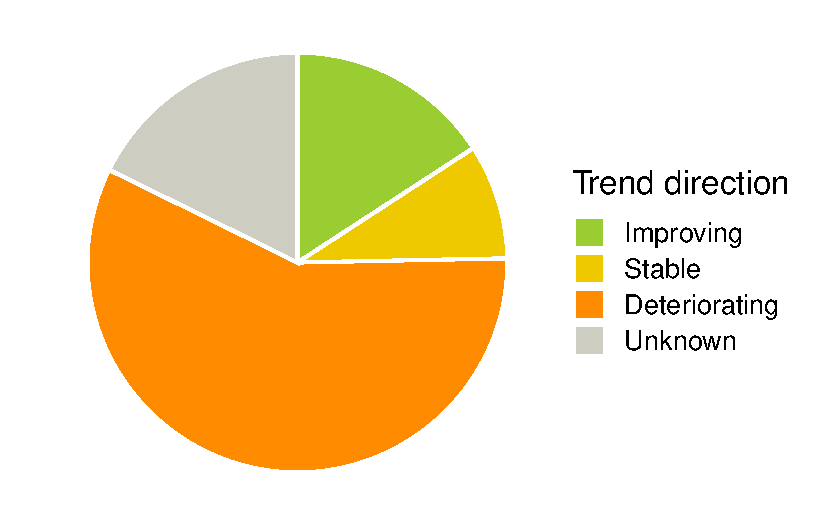
\includegraphics[keepaspectratio]{analyse_data_main_files/figure-pdf/qualifiers_1a-1.pdf}}

\end{minipage}%
%
\begin{minipage}{0.50\linewidth}

\pandocbounded{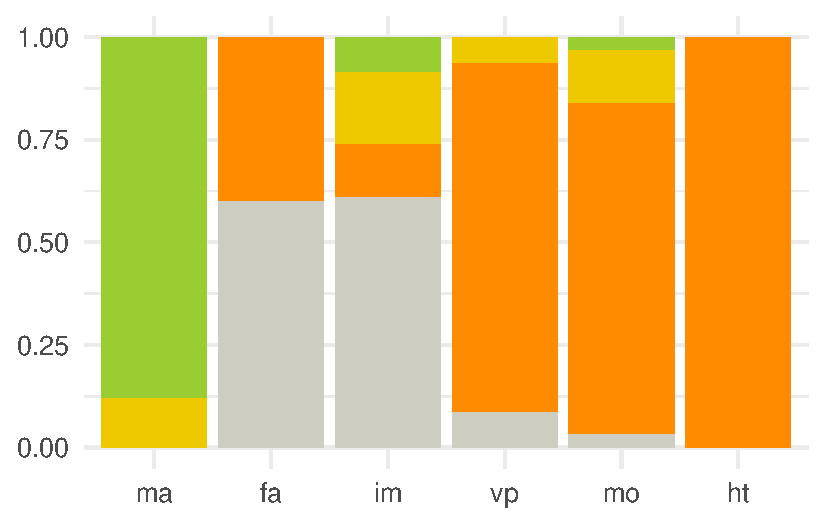
\includegraphics[keepaspectratio]{analyse_data_main_files/figure-pdf/qualifiers_1b-1.pdf}}

\end{minipage}%
\newline
\begin{minipage}{0.29\linewidth}

\pandocbounded{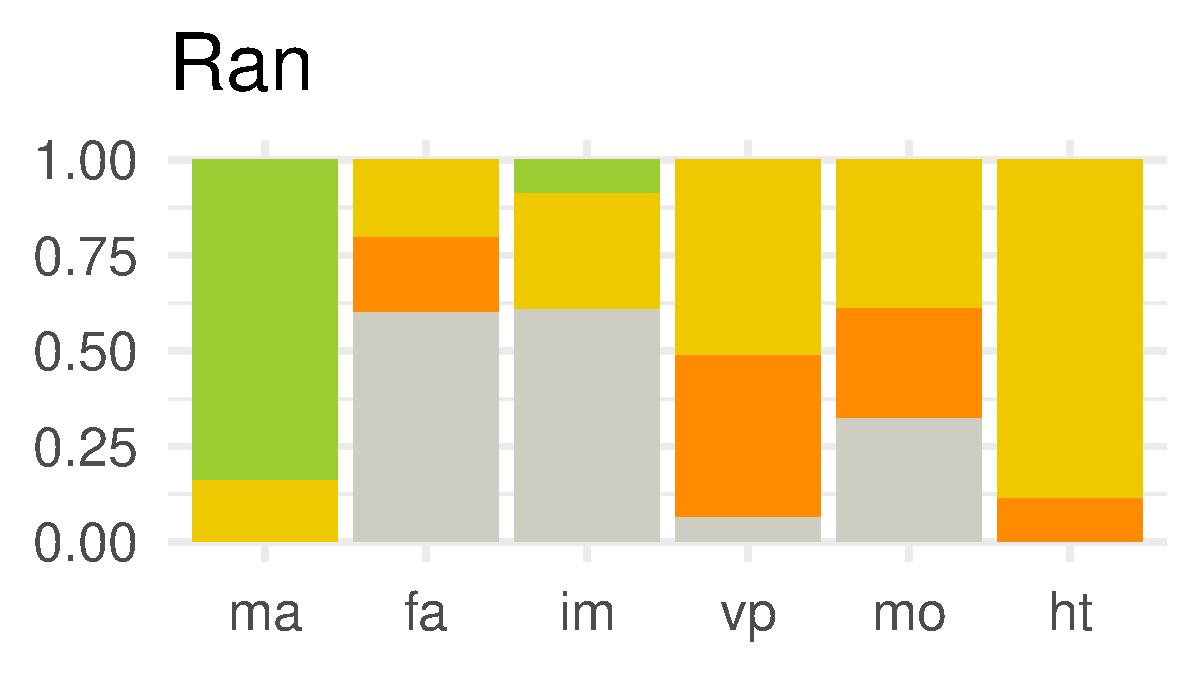
\includegraphics[keepaspectratio]{analyse_data_main_files/figure-pdf/qualifiers_2_ran_calc-1.pdf}}

\end{minipage}%
%
\begin{minipage}{0.25\linewidth}

\pandocbounded{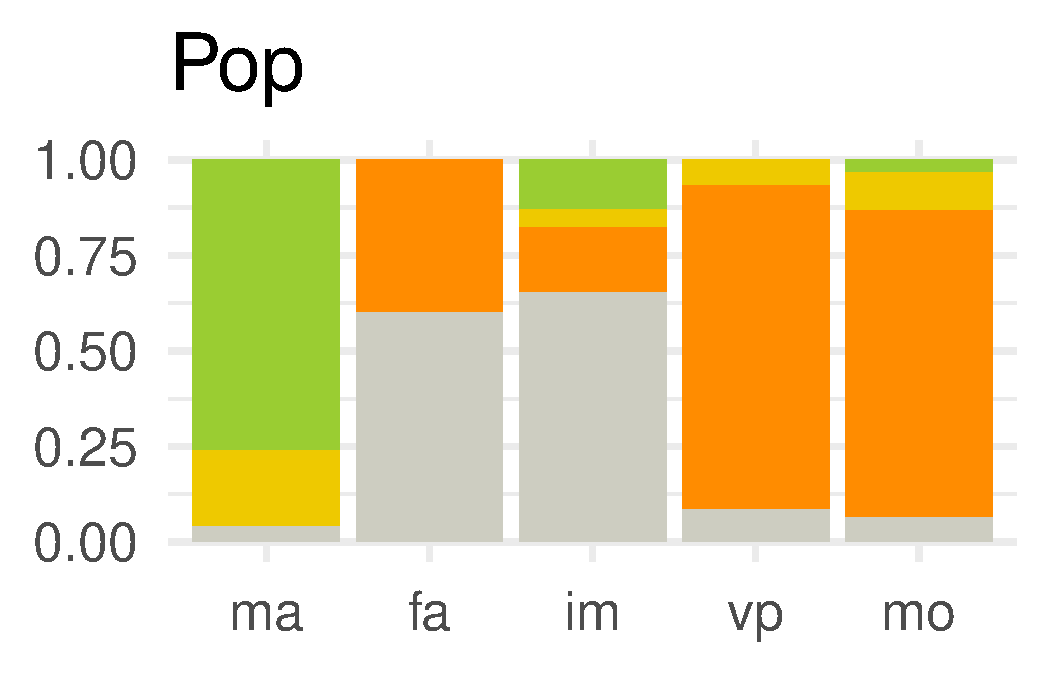
\includegraphics[keepaspectratio]{analyse_data_main_files/figure-pdf/qualifiers_2_pop-1.pdf}}

\end{minipage}%
%
\begin{minipage}{0.11\linewidth}

\pandocbounded{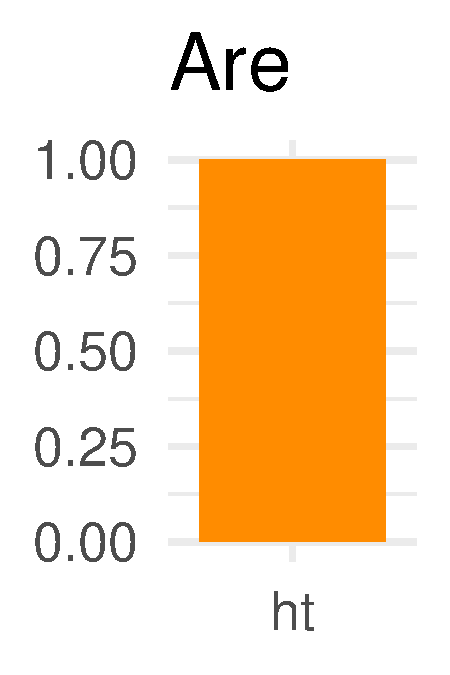
\includegraphics[keepaspectratio]{analyse_data_main_files/figure-pdf/qualifiers_2_are-1.pdf}}

\end{minipage}%
%
\begin{minipage}{0.25\linewidth}

\pandocbounded{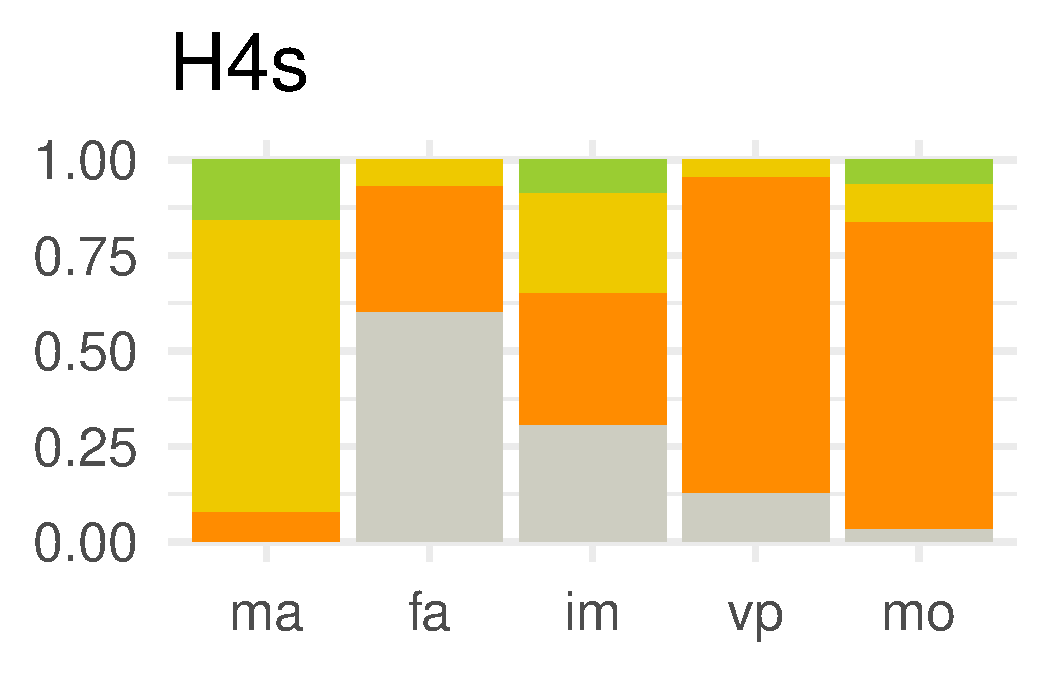
\includegraphics[keepaspectratio]{analyse_data_main_files/figure-pdf/qualifiers_2_h4s-1.pdf}}

\end{minipage}%
%
\begin{minipage}{0.11\linewidth}

\pandocbounded{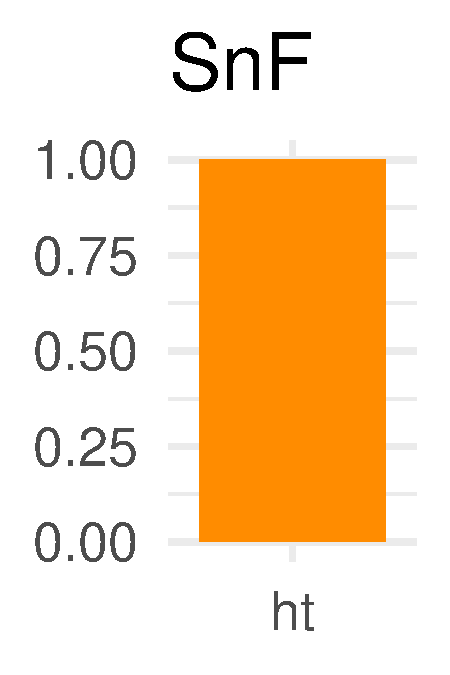
\includegraphics[keepaspectratio]{analyse_data_main_files/figure-pdf/qualifiers_2_snf-1.pdf}}

\end{minipage}%

\caption{\label{fig-trend-qualifiers}Overall short-term (2013-2024)
trends identified during the 2025 assessments. Top row: the overall
``\emph{trend qualifiers}'' among all assessments (pie chart) and the
distribution of trend types across the main groups of features
(columns). Bottom row: short term trends for the main assessment
parameters. (ma: mammals, fa= fishes \& amphibians, im= insects and
molluscs, vp: vascular plants, mo: mosses, ht: habitat types; Ran:
range, Pop: population, Are: area, H4s: habitat for species, SnF:
structure and function)}

\end{figure}%

\subsubsection{Long term trends}\label{long-term-trends}

In this reporting round, \emph{long-term trends} were only assessed for
some of the parameters (range \& population size for species, and range
and area for habitat types), and only in cases when the expert were
long-term evidence was available. These cases means that\ldots{}
\ldots{} \textbf{?@tbl-xxxx} provides an overview of the

\subsubsection{Changes since 2019}\label{changes-since-2019}

The 2019 reporting period was the first reporting period for Norway
under Resolution 8 of the Bern Convention. This reporting period was
considered to be a pilot exercise by the Bern Convention Secretariat, so
only very few species and habitat types were selected for reporting.
Table~\ref{tbl-changes-sp} provides an overview of the changes in the
overall assessment conclusions for the overlapping species.

\begin{table}

\caption{\label{tbl-changes-sp}}

\centering{

\centering
\caption{\label{tab:tbl-changes-sp}Changes in the overall conclusions of the repeated assessments between 2019 and 2025 (FV: Favourable; U1: Unfavourable - inadequate; U2: Unfavourable - bad; XX: Unknown)}
\centering
\begin{tabular}[t]{c|c|l}
\hline
Change & N & Assessments\\
\hline
U1 --> U1 & 5 & Gulflekktorvlibelle (ATL); marisko (ALP, ATL, BOR); rikmyr (ALP)\\
\hline
U2 --> U2 & 5 & Alvemose (ATL, BOR); eremitt (BOR); rikmyr (ATL, BOR)\\
\hline
FV --> U1 & 4 & Oter (ALP, ARC, ATL, BOR)\\
\hline
XX --> U1 & 4 & Brunbjørn (ALP, BOR); ulv (ALP, BOR)\\
\hline
U1 --> U2 & 3 & Alvemose (ALP); edellauvskog (ATL, BOR)\\
\hline
XX --> XX & 3 & Bekkeniøye (ATL, BOR); smalknøttsnegl (BOR)\\
\hline
U2 --> U1 & 2 & Myrsildre (ALP, ATL)\\
\hline
FV --> XX & 1 & Hvitfinnet steinulk (BOR)\\
\hline
U1 --> FV & 1 & Gulflekktorvlibelle (BOR)\\
\hline
\end{tabular}

}

\end{table}%

TODO: reasons for change\ldots{}

\subsection{Background factors}\label{background-factors}

\subsubsection{Key pressures}\label{key-pressures}

TBC \ldots{}

\subsubsection{Main conservation
measures}\label{main-conservation-measures}

TBC \ldots{}

\subsubsection{Role of the Emerald
Network}\label{role-of-the-emerald-network}

Protected areas, and in particular the Emerald Network is assumed to
provide substantial support for endangered species and habitats. Several
parts of the Bern assessment explore the influence of the Emerald
Network, thus providing useful feedback for conservation management. In
Table~\ref{tbl-eme-trends} we compare \emph{within Emerald} short-term
trends of several parameters with the general trends of the same
parameters within the entire biogeographic region. This comparison is
only sensitive to the direction of the trend, so significant differences
between slight and drastic declines (or improvements) can still be
marked as ``same within/beyond Emerald'' in Table~\ref{tbl-eme-trends}.

\begin{table}

\caption{\label{tbl-eme-trends}}

\centering{

\centering
\caption{\label{tab:tbl-eme-trends}Comparison of short term trends in several parameters within the Emerald network and outside of it.}
\centering
\begin{tabular}[t]{l|c|c|c|c}
\hline
\multicolumn{1}{c|}{ } & \multicolumn{2}{c|}{Species parameters} & \multicolumn{2}{c}{Habitat parameters} \\
\cline{2-3} \cline{4-5}
Trends within/beyond Emerald & Area of habitats (Are) & Habitat for species (H4s) & Population (Pop) & Structure and function (SnF)\\
\hline
Better *within* Emerald & 15 & 2 & 1 & 13\\
\hline
Same trend within/beyond & 2 & 84 & 72 & 4\\
\hline
Better *beyond* Emerald & - & 1 & 3 & -\\
\hline
Unknown (at least partly) & - & 54 & 65 & -\\
\hline
\end{tabular}

}

\end{table}%

TODO: comparison of conservation measures within/beyond Emerald\ldots{}

\subsection{Fjellrev: a success story}\label{fjellrev-a-success-story}

TBC\ldots{}

\subsection{Data availability}\label{data-availability}

(?) TBD/TBC\ldots{}

\subsection{References}\label{references}

\subsection{Annexes}\label{annexes}

\begin{itemize}
\tightlist
\item
  A table with all species \& habitats (incl latin names) and their main
  conclusions
\item
  (??) A list of simple ``conclusion figures'' for each species \&
  habitat (one per page)
\end{itemize}




\end{document}
